%%%%(c)
%%%%(c)  This file is a portion of the source for the textbook
%%%%(c)
%%%%(c)    Abstract Algebra: Theory and Applications
%%%%(c)    Copyright 1997 by Thomas W. Judson
%%%%(c)
%%%%(c)  See the file COPYING.txt for copying conditions
%%%%(c)
%%%%(c)
\chap{Homomorphisms}{homomorph}

%% TWJ, 2010/03/31
%% The chapter HOMOMORPHISMS AND FACTOR GROUPS is now
%% two chapters: (10) NORMAL SUBGROUPS AND FACTOR GROUPS
%% (11) HOMOMORPHISMS
 
\section{Group Homomorphisms}
 
 
One of the basic ideas of algebra is the concept of a homomorphism, a
natural generalization of an isomorphism. If we relax the requirement
that an isomorphism of groups be bijective, we have a homomorphism.  A
\boldemph{homomorphism}\index{Group!homomorphism of}\index{Homomorphism!of
groups} between groups $(G, \cdot)$ and $(H, \circ)$ is a map $\phi :
G \rightarrow H$ such that  
\[
\phi( g_1 \cdot g_2 ) = \phi( g_1 ) \circ \phi( g_2 )
\]
for $g_1, g_2 \in G$. The range of $\phi$ in $H$ is called the \boldemph{
homomorphic image}\index{Homomorphic image}~of~$\phi$.
 
 
Two groups are related in the strongest possible way if they are
isomorphic; however, a weaker relationship may exist between two
groups.  For example, the symmetric group $S_n$ and the group ${\mathbb
Z}_2$ are related by the fact that $S_n$ can be divided into even and
odd permutations that exhibit a group structure like that ${\mathbb
Z}_2$, as shown in the following multiplication table. 
\begin{center}
\begin{tabular}{c|cc}
            & even & odd \\
\hline
even & even & odd \\
odd  & odd  & even
\end{tabular}
\end{center}
We use homomorphisms to study relationships such as the one we have
just described.
 
 
\begin{example}{homo_Zn}
Let $G$ be a group and $g \in G$. Define a map $\phi : {\mathbb Z}
\rightarrow G$ by $\phi( n ) = g^n$. Then $\phi$ is a group
homomorphism, since 
\[
\phi( m + n ) = g^{ m + n} = g^m g^n = \phi( m ) \phi( n ).
\]
This homomorphism maps ${\mathbb Z}$ onto the cyclic subgroup of $G$
generated by $g$. 
\mbox{\hspace*{1in}}
\end{example}
 
 
\begin{example}{homo_GL2}
Let $G = GL_2( {\mathbb R })$. If
\[
A=
\begin{pmatrix}
a & b \\
c & d
\end{pmatrix}
\]
is in $G$, then the determinant is  nonzero; that is, $\det(A) = ad -bc
\neq 0$.  Also, for any two elements $A$ and $B$ in $G$, $\det(AB) =
\det(A) \det(B)$. Using the determinant, we can define a homomorphism
$\phi : GL_2( {\mathbb R }) \rightarrow {\mathbb R}^\ast$ by
$A~\mapsto~\det(A)$.  
\mbox{\vspace{1in}}
\end{example}
 
 
\begin{example}{homo_T}
Recall that the circle group ${ \mathbb T}$ consists of all complex
numbers $z$ such that $|z|=1$. We can define a homomorphism $\phi$
from the additive group of real numbers ${\mathbb R}$ to ${\mathbb T}$ by
$\phi : \theta \mapsto \cos \theta + i \sin \theta$. Indeed, 
\begin{align*}
\phi( \alpha + \beta )
& =
\cos( \alpha + \beta ) + i \sin( \alpha + \beta ) \\
& =
(\cos \alpha \cos \beta - \sin \alpha \sin \beta)  + i( \sin \alpha 
\cos \beta + \cos \alpha \sin \beta ) \\
& =
(\cos \alpha + i \sin \alpha ) + (\cos \beta + i \sin \beta
) \\
& = \phi( \alpha ) \phi( \beta ).
\end{align*}
Geometrically, we are simply wrapping the real line around the circle 
in a group-theoretic fashion. 
\end{example}

 
The following proposition lists some basic properties of group
homomorphisms.
 
 
\begin{proposition}\label{HomorphismSubgroupProp}
Let $\phi : G_1 \rightarrow G_2$ be a homomorphism of groups. Then 
\begin{enumerate}
 
\rm \item \it
If $e$ is the identity of $G_1$, then $\phi( e)$ is the identity of
$G_2$;  
 
\rm \item \it
For any element $g \in G_1$, $\phi( g^{-1}) = [\phi( g )]^{- 1}$;
 
\rm \item \it
If $H_1$ is a subgroup of $G_1$, then $\phi( H_1 )$ is a subgroup of
$G_2$;
 
\rm \item \it
If $H_2$ is a  subgroup of $G_2$, then $\phi^{-1}(H_2) = \{ g \in G _1:
\phi(g) \in H_2 \}$ is a subgroup of $G_1$. Furthermore, if $H_2$ is
normal in $G_2$, then $\phi^{-1}(H_2)$ is normal in $G_1$. 

%% TWJ, 2011/09/15
%% Changed G to G_1
%% Suggested by Tony Perkins
 
\end{enumerate}
\end{proposition}
 
 
\begin{proof}
(1)
Suppose that $e$ and $e'$ are the identities of $G_1$ and $G_2$,
respectively; then
\[
e' \phi(e) = \phi(e) = \phi(e e) = \phi(e) \phi(e).
\]
By cancellation, $\phi(e) = e'$.
 
 
(2)
This statement follows from the fact that
\[
\phi( g^{-1}) \phi(g) = \phi(g^{-1} g) = \phi(e) = e'.
\]
 
 % Corrected notation error.  Suggested by P. Diethelm.  TWJ 16/8/2013.


(3)
The set $\phi(H_1)$ is nonempty since the identity of $G_2$ is in
$\phi(H_1)$.
Suppose that $H_1$ is a subgroup of $G_1$ and let $x$ and $y$ be in
$\phi(H_1)$. There exist elements $a, b \in H_1$ such that $\phi(a) =
x$ and $\phi(b)=y$. Since 
\[
xy^{-1} = \phi(a)[ \phi(b)]^{-1} = \phi(a b^{-1} ) \in \phi(H_1),
\]
$\phi(H_1)$ is a subgroup of $G_2$ by Proposition~\ref{groups:subgroup_prop}.
%H_2 changed to G_2 in proof.  Suggested by K. Wenholz.
%TWJ - 12/19/2011
 
 
(4)
Let $H_2$ be a subgroup of $G_2$ and define $H_1$ to be
$\phi^{-1}(H_2)$; that is, $H_1$ is the set of all $g \in G_1$ such
that $\phi(g) \in H_2$.  The identity is in $H_1$ since $\phi(e) = e'$.
If $a$ and $b$ are in $H_1$, then $\phi(ab^{-1}) = \phi(a)[ \phi(b)
]^{-1}$ is in $H_2$ since $H_2$ is a subgroup of $G_2$.  Therefore,
$ab^{-1} \in H_1$ and $H_1$ is a subgroup of $G_1$. If $H_2$ is normal
in $G_2$, we must show that $g^{-1} h g \in H_1$ for $h \in H_1$ and
$g \in G_1$. But 
\[
\phi( g^{-1} h g) = [ \phi(g) ]^{-1} \phi( h ) \phi( g ) \in
H_2,
\]
since $H_2$ is a normal subgroup of $G_2$.  Therefore, $g^{-1}hg \in
H_1$.
\end{proof}
 
 
\medskip
 
 
Let $\phi : G \rightarrow H$ be a group homomorphism and suppose that
$e$ is the identity of $H$. By Proposition~\ref{HomorphismSubgroupProp}, $\phi^{-1} ( \{ e \}
)$ is a subgroup of $G$. This subgroup is called the \boldemph{
kernel}\index{Kernel!of a group
homomorphism}\index{Homomorphism!kernel of a group} of $\phi$ and will
be denoted by $\ker \phi$\label{kernelofphi}.  In fact, this subgroup
is a normal subgroup of $G$ since the trivial subgroup is normal in
$H$.  We state this result in the following theorem, which says that
with every homomorphism of groups we can naturally associate a normal
subgroup.   
 
 
\begin{theorem}
Let $\phi : G \rightarrow H$ be a group homomorphism. Then the kernel
of $\phi$ is a normal subgroup of $G$. 
\end{theorem}
 
 
\begin{example}{homo_G2_to_R}
Let us examine the homomorphism $\phi : GL_2( {\mathbb R }) \rightarrow
{\mathbb R}^\ast$ defined by $A \mapsto \det( A )$. Since 1 is the
identity of ${\mathbb R}^\ast$, the kernel of this homomorphism is all
$2 \times 2$ matrices having determinant one. That is, $\ker \phi =
SL_2( {\mathbb R })$.
\mbox{\hspace{1in}}
\end{example}
 
 
\begin{example}{kernel}
The kernel of the group homomorphism $\phi : {\mathbb R} \rightarrow
{\mathbb C}^\ast$ defined by $\phi( \theta ) = \cos \theta + i \sin
\theta$ is $\{ 2 \pi n : n \in {\mathbb Z} \}$. Notice that $\ker \phi
\cong {\mathbb Z}$. 
\end{example}
 
 
\begin{example}{homo_Z7}
Suppose that we wish to determine all possible homomorphisms $\phi$
from ${\mathbb Z}_7$ to  ${\mathbb Z}_{12}$. Since the kernel of $\phi$ must
be a subgroup of  ${\mathbb Z}_7$, there are only two possible
kernels, $\{ 0 \}$ and all of ${\mathbb Z}_7$.  The image of a subgroup
of ${\mathbb Z}_7$ must be a subgroup of ${\mathbb Z}_{12}$. Hence, there is
no injective homomorphism; otherwise, ${\mathbb Z}_{12}$ would have a
subgroup of order 7, which is impossible. Consequently, the only
possible homomorphism from ${\mathbb Z}_7$ to  ${\mathbb Z}_{12}$ is the one
mapping all elements to zero. 
\end{example}
 
 
\begin{example}{homo_g^n}
Let $G$ be a group. Suppose that  $g \in G$ and $\phi$ is the
homomorphism from ${\mathbb Z}$ to $G$ given by $\phi( n ) = g^n$. If the
order of $g$ is infinite, then the kernel of this homomorphism is $\{
0 \}$ since $\phi$ maps ${\mathbb Z}$ onto the cyclic subgroup of $G$
generated by $g$. However, if the order of $g$ is finite, say $n$,
then the kernel of $\phi$ is $n {\mathbb Z}$.
\end{example}
 

 
 
 
\section{The Isomorphism Theorems}
 
 
Though at first it is not evident that factor groups correspond
exactly to homomorphic images, we can use factor groups to study
homomorphisms. We already know that with every group homomorphism
$\phi: G \rightarrow H$ we can associate a normal subgroup of $G$,
$\ker \phi$; the converse is also true. Every normal subgroup of a
group $G$ gives rise to homomorphism of groups. 
 
Let $H$ be a normal subgroup of $G$. Define the \boldemph{
natural}\index{Homomorphism!natural} or \boldemph{canonical
homomorphism}\index{Homomorphism!canonical}  
\[
\phi : G \rightarrow G/H
\]
by
\[
\phi(g) = gH.
\]
This is indeed a homomorphism, since
\[
\phi( g_1 g_2 ) = g_1 g_2 H =  g_1 H g_2 H = \phi( g_1) \phi( g_2 ). 
\]
The kernel of this homomorphism is $H$.	 The following theorems 
describe the relationships among group homomorphisms, normal 
subgroups, and factor groups. 
 
 
\begin{theorem}[First Isomorphism Theorem]\label{FirstIsoTheorem}\index{First Isomorphism Theorem!for groups}
If $\psi : G \rightarrow H$ is a group homomorphism with $K =\ker
\psi$, then $K$ is normal in $G$. Let $\phi: G \rightarrow G/K$ be
the canonical homomorphism.  Then there exists a unique isomorphism
$\eta: G/K \rightarrow \psi(G)$ such that $\psi =  \eta \phi$.
\end{theorem}
 
 % Proof rewritten for clarification.  Suggested by P. Diethelm.  TWJ 16/8/2013.
 
\begin{proof}
We already know that $K$ is normal in $G$. Define $\eta: G/K
\rightarrow \psi(G)$ by $\eta(gK) = \psi(g)$.  We first show that
$\eta$ is a well-defined map.  If $g_1 K =g_2 K$, then for some $k \in
K$, $g_1 k=g_2$; consequently, 
\[
\eta(g_1 K) = \psi(g_1) = \psi(g_1) \psi(k) = \psi(g_1k) = \psi(g_2)
= \eta(g_2 K). 
\]
Thus, $\eta$ does not depend on the choice of coset representatives and the map $\eta: G/K \rightarrow \psi(G)$  is uniquely defined since $\psi =  \eta \phi$.
We must also
show that $\eta$ is a homomorphism, but 
\begin{align*}
\eta( g_1K g_2K ) & = \eta(g_1 g_2K) \\
& = \psi(g_1 g_2) \\
& = \psi(g_1) \psi(g_2) \\
& = \eta( g_1K) \eta( g_2K ).
\end{align*}
Clearly, $\eta$ is onto $\psi( G)$. 
To show that $\eta$ is one-to-one, suppose that $\eta(g_1 K) = 
\eta(g_2 K)$. Then $\psi(g_1) = \psi(g_2)$. This implies that 
$\psi( g_1^{-1} g_2 ) = e$, or $g_1^{-1} g_2$ is in the kernel of $\psi$; 
hence, $g_1^{-1} g_2K = K$; that is, $g_1K =g_2K$.  
\end{proof}
 
 
\medskip
 
 
Mathematicians often use diagrams called \boldemph{commutative
diagrams}\index{Commutative diagrams} to describe such theorems. The
following diagram ``commutes'' since $\psi = \eta \phi$. 



\begin{center}
\tikzpreface{homomorphs_first_isomorphism}
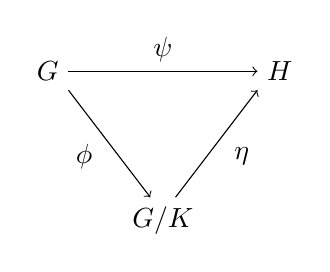
\begin{tikzpicture}[scale=0.8]

\node at (1.5,2) [above] {$\psi$};
\node at (0.25,0.65) {$\phi$};
\node at (2.75,0.65) {$\eta$};
\draw [->] (0,2)  node [left] {$G$} -- (3,2) node [right] {$H$};
\node at (1.5,0) [below] {$G/K$};
\draw [->] (0,1.7) -- (1.3,0);
\draw [->] (1.7,0) -- (3,1.7);


\end{tikzpicture}

\end{center}

 
 
\begin{example}{homo_cyclic}
Let $G$ be a cyclic group with generator $g$. Define a map $\phi :
{\mathbb Z} \rightarrow G$ by $n \mapsto g^n$.  This map is a surjective
homomorphism since  
\[
\phi( m + n) = g^{m+n} = g^m g^n = \phi(m) \phi(n).
\]
Clearly $\phi$ is onto. If $|g| = m$, then  $g^m = e$. Hence, $\ker
\phi = m {\mathbb Z}$ and ${\mathbb Z} / \ker \phi =  {\mathbb Z} / m {\mathbb Z}
\cong G$. On the other hand, if the order of $g$ is infinite, then
$\ker \phi = 0$ and $\phi$ is an isomorphism of $G$ and ${\mathbb Z}$.
Hence, two cyclic groups are isomorphic exactly when they have the
same order. Up to isomorphism, the only cyclic groups are ${\mathbb Z}$
and ${\mathbb Z}_n$. 
\end{example}
 
 
\begin{theorem}[Second Isomorphism Theorem]\label{homomorph:theorem:2nd_isomorph}\index{Second Isomorphism
Theorem! for groups}
Let  $H$ be a subgroup of a group $G$ (not necessarily normal in $G$)
and $N$ a normal subgroup of $G$.  Then $HN$ is a subgroup of $G$,
$H \cap N$ is a normal subgroup of $H$, and 
\[
H / H \cap N \cong HN /N.
\]
\end{theorem}
 
 
\begin{proof}
We will first show that $HN = \{ hn : h \in H, n \in N \}$ is a
subgroup of $G$.  Suppose that  $h_1 n_1, h_2 n_2 \in HN$. Since 
$N$ is normal, $(h_2)^{-1} n_1 h_2 \in N$. So 
\[
(h_1 n_1)(h_2 n_2) = h_1 h_2 ( (h_2)^{-1} n_1 h_2 )n_2
\]
is in $HN$. The inverse of $hn \in HN$ is in $HN$ since
\[
( hn )^{-1} = n^{-1 } h^{-1} = h^{-1} (h n^{-1} h^{-1} ).
\]
 
 
Next, we prove that $H \cap N$ is normal in $H$. Let $h \in H$ and $n
\in H \cap N$. Then $h^{-1} n h \in H$ since each element is in $H$.
Also, $h^{-1} n h \in N$ since $N$ is normal in $G$; therefore,
$h^{-1} n h \in H \cap N$. 
 
 
Now define a map $\phi$ from $H$ to $ HN / N$ by $h \mapsto h N$. The
map $\phi$ is onto, since any coset $h n N = h N$ is the image of $h$
in $H$. We also know that $\phi$ is a homomorphism because 
\[
\phi( h  h')  = h h' N =  h N h' N =  \phi( h ) \phi( h').
\]
By the First Isomorphism Theorem, the image of $\phi$ is isomorphic to
$H / \ker \phi$; that is,
\[
HN/N = \phi(H) \cong H / \ker \phi.
\]
Since
\[
\ker \phi = \{ h \in H : h \in N \} = H \cap N,
\]
$HN/N = \phi(H) \cong H / H \cap N$.
\end{proof}
 
 
\begin{theorem}[Correspondence Theorem]\label{CorrespondTheorem}\index{Correspondence Theorem!for groups}
Let $N$ be a normal subgroup of a group $G$. Then $H \mapsto H/N$
is a one-to-one correspondence between the set of subgroups $H$
containing $N$  and the set of subgroups of $G/N$. Furthermore, the
normal subgroups of $G$ containing $N$ correspond to normal subgroups of~$G/N$. 
\end{theorem}

 % Statement of the Correspondence Theorem corrected.  Suggested by P. Diethelm.  TWJ 16/8/2013.
 
 
\begin{proof}
Let $H$ be a subgroup of $G$ containing $N$. Since $N$ is normal in
$H$, $H/N$ makes sense.  Let $aN$ and $bN$ be elements of $H/N$. Then
$(aN)( b^{-1} N )= ab^{-1}N \in H/N$; hence, $H/N$ is a subgroup of
$G/N$. 


Let $S$ be a subgroup of $G/N$. This subgroup is a set of cosets of
$N$.  If  $H= \{ g \in G : gN \in S \}$, then for $h_1, h_2 \in H$, we
have that $(h_1 N)( h_2 N )= h_1 h_2 N \in S$ and $h_1^{-1} N \in S$.
Therefore, $H$ must be a subgroup of $G$. Clearly, $H$ contains $N$.
Therefore, $S = H / N$. Consequently, the map  $H \mapsto H/N$ is
onto. 

% Notation error corrected.  Suggested by P. Diethelm.  TWJ 16/8/2013.
    
Suppose that $H_1$ and $H_2$ are subgroups of $G$ containing $N$ such
that $H_1/N = H_2/N$. If $h_1 \in H_1$, then $h_1 N \in H_1/N$. Hence,
$h_1 N = h_2 N \subset H_2$ for some $h_2$ in $H_2$. However, since
$N$ is contained in $H_2$, we know that $h_1 \in H_2$ or $H_1 \subset
H_2$. Similarly, $H_2 \subset H_1$.  Since $H_1 = H_2$, the map  $H
\mapsto H/N$ is one-to-one. 

%H/N changed to N/H.  Suggested by S. Engle.
%TWJ - 12/19/2011

%Changed it back.  What was I thinking?  Suggested by R. Beezer.
%TWJ - 11/29/2012


 
Suppose that $H$ is normal in $G$ and $N$ is a subgroup of $H$.  Then
it is easy to verify that the map $G/N \rightarrow G/H$ defined by $gN
\mapsto gH$ is  a homomorphism.  The kernel of this homomorphism is
$H/N$, which proves that $H/N$ is normal in $G/N$. 
 
 
Conversely, suppose that $H/N$ is normal in $G/N$. The homomorphism
given by 
\[
G \rightarrow G/N \rightarrow \frac{G/N}{H/N}
\]
has kernel $H$. Hence, $H$ must be normal in $G$.
\end{proof}
 
\medskip
 
 
Notice that in the course of the proof of Theorem~\ref{CorrespondTheorem}, we have also
proved the following theorem. 
 
 
\begin{theorem}[Third Isomorphism Theorem]\label{ThirdIsoTheorem}\index{Third Isomorphism Theorem!for groups}
Let $G$ be a group and $N$ and $H$ be normal subgroups of $G$ with $N
\subset H$.  Then 
\[
G/H \cong \frac{G/N}{H/N}.
\]
\end{theorem}
 
 
\begin{example}{3rd_isomorph}
By the Third Isomorphism Theorem,
\[
{\mathbb Z} / m {\mathbb Z} \cong ({\mathbb Z}/ mn {\mathbb Z})/ (m {\mathbb Z}/ mn
{\mathbb Z}). 
\]
Since $| {\mathbb Z} / mn {\mathbb Z} | = mn$ and  $|{\mathbb Z} / m{\mathbb Z}| =
m$, we have $| m {\mathbb Z} / mn {\mathbb Z}| = n$. 
\end{example}
 
 
\markright{EXERCISES}
\section*{Exercises}
\exrule
 
 
 
{\small
 
 
\begin{enumerate}
 
 
 
\item
Prove that $\det( AB) = \det(A) \det(B)$ for $A, B \in GL_2( {\mathbb R}
)$. This shows that the determinant is a homomorphism from $GL_2(
{\mathbb R} )$ to ${\mathbb R}^*$. 
 
 
 
\item
Which of the following maps are homomorphisms? If the map is a
homomorphism, what is the kernel? 
\begin{enumerate}
 
 \item
$\phi : {\mathbb R}^\ast \rightarrow GL_2 ( {\mathbb R})$ defined by
\[
\phi( a ) =
\begin{pmatrix}
1 & 0 \\
0 & a
\end{pmatrix}
\]
 
 \item
$\phi : {\mathbb R} \rightarrow GL_2 ( {\mathbb R})$ defined by
\[
\phi( a ) =
\begin{pmatrix}
1 & 0 \\
a & 1
\end{pmatrix}
\]
 
 \item
$\phi : GL_2 ({\mathbb R})   \rightarrow {\mathbb R}$ defined by
\[
\phi
\left(
\begin{pmatrix}
a & b \\
c & d
\end{pmatrix}
\right)
= a + d
\]
 
 \item
$\phi : GL_2 ( {\mathbb R})   \rightarrow {\mathbb R}^\ast$ defined by 
\[
\phi
\left(
\begin{pmatrix}
a & b \\
c & d
\end{pmatrix}
\right)
= ad -bc
\]
 
 \item
$\phi : {\mathbb M}_2( {\mathbb R})   \rightarrow {\mathbb R}$ defined by
\[
\phi
\left(
\begin{pmatrix}
a & b \\
c & d
\end{pmatrix}
\right)
= b,
\]
where ${\mathbb M}_2( {\mathbb R})$ is the additive group of $2 \times 2$ matrices with entries in ${\mathbb R}$.
 
\end{enumerate}
 
  
 
\item
Let $A$ be an $m \times n$ matrix.  Show that matrix multiplication,
$x \mapsto Ax$, defines a homomorphism $\phi : {\mathbb R}^n \rightarrow
{\mathbb R}^m$. 
 
 
\item
Let $\phi : {\mathbb Z} \rightarrow {\mathbb Z}$ be given by $\phi(n) = 7n$.
Prove that $\phi$ is a group homomorphism. Find the kernel and the
image of $\phi$.
 
 
\item
Describe all of the homomorphisms from ${\mathbb Z}_{24}$ to ${\mathbb Z}_{18}$. 
 
 
\item
Describe all of the homomorphisms from ${\mathbb Z}$ to ${\mathbb Z}_{12}$. 
 
 
\item
In the group ${\mathbb Z}_{24}$, let $H = \langle 4 \rangle$ and $N =
\langle 6 \rangle$. 
\begin{enumerate}
 
 \item
List the elements in $HN$ (we usually write $H + N$ for these additive
groups) and $H \cap N$. 
 
 \item
List the cosets in $HN/N$, showing the elements in each coset.
 
 \item
List the cosets in $H/(H \cap N)$, showing the elements in each coset. 
 
 \item
Give the correspondence between $HN/N$ and $H/(H \cap N)$ described in
the proof of the Second Isomorphism Theorem. 
 
\end{enumerate}
 
 
%***************************THEORY******************
 
 
\item
If $G$ is an abelian group and $n \in {\mathbb N}$, show that $\phi : G
\rightarrow G$  defined by $g \mapsto g^n$ is a group homomorphism. 
 
 

 
\item
If $\phi : G \rightarrow H$ is a group homomorphism and $G$ is
abelian, prove that $\phi(G)$ is also abelian. 
 
 
\item
If $\phi : G \rightarrow H$ is a group homomorphism and $G$ is cyclic,
prove that $\phi(G)$ is also cyclic. 
 
 
\item
Show that a homomorphism defined on a cyclic group is completely
determined by its action on the generator of the group.


 
 
\item
Let $G$ be a group of order $p^2$, where $p$ is a prime number. If $H$
is a subgroup of $G$ of order $p$, show that $H$ is normal in $G$.
Prove that $G$ must be abelian. 
 
 
\item
If a group $G$ has exactly one subgroup $H$ of order $k$, prove that
$H$ is normal in $G$. 
 
 
\item
Prove or disprove: ${\mathbb Q} / {\mathbb Z} \cong {\mathbb Q}$.
 
 
%\item
%Define the \boldemph{centralizer}\index{Element!centralizer
%of}\index{Centralizer!of an element} of an element $g$ in a group $G$
%to be the set  
%\[
%C(g) = \{ x \in G : xg = gx \}.
%\]
%Show that $C(g)$ is a subgroup of $G$.  If $g$ generates a normal
%subgroup of $G$, prove that $C(g)$ is normal in $G$.
% 
% 
%\item
%Recall that the \boldemph{center}\index{Group!center of} of a group $G$ is
%the set 
%\[
%Z(G) = \{ x \in G : xg = gx \mbox{ for all $g \in G$ } \}.
%\]
%\begin{enumerate}
% 
% \item
%Calculate the center of $S_3$.
% 
% \item
%Calculate the center of $GL_2 ( {\mathbb R} )$.
% 
% \item
%Show that the center of any group $G$ is a normal subgroup of $G$. 
% 
% \item
%If $G / Z(G)$ is cyclic, show that $G$ is abelian.
% 
%\end{enumerate}
% 
 
\item
Let $G$ be a finite group and $N$ a normal subgroup of $G$. If $H$ is
a subgroup of $G/N$, prove that $\phi^{-1}(H)$ is a subgroup in $G$ of
order $|H| \cdot |N|$, where $\phi : G \rightarrow G/N$ is the
canonical homomorphism. 
 
 
%\item
%Let $G$ be a group and let $G' = \langle aba^{- 1} b^{-1} \rangle$;
%that is, $G'$ is the subgroup of all finite products of elements in
%$G$ of the form $aba^{-1}b^{-1}$.  The subgroup $G'$ is called the
%\boldemph{commutator
%subgroup}\index{Subgroup!commutator}\label{commutatorsubgroup} of $G$.  
%\begin{enumerate}
% 
% \item
%Show that $G'$ is a normal subgroup of $G$.
%
% \item
%Let $N$ be  a normal subgroup of $G$.  Prove that $G/N$ is abelian if
%and only if $N$ contains the commutator subgroup of $G$.
% 
%\end{enumerate}

 
\item
Let $G_1$ and $G_2$ be groups, and let $H_1$ and $H_2$ be normal subgroups
of $G_1$ and $G_2$ respectively. Let $\phi : G_1 \rightarrow G_2$ be a
homomorphism. Show that $\phi$ induces a natural homomorphism
$\overline{\phi} : (G_1/H_1) \rightarrow (G_2/H_2)$ if $\phi(H_1) \subseteq
H_2$. 
 
 
\item
If $H$ and $K$ are normal subgroups of $G$ and $H \cap K = \{ e \}$,
prove that $G$ is isomorphic to a subgroup of $G/H \times G/K$.
 
 
 
\item
Let $\phi : G_1 \rightarrow G_2$ be a surjective group homomorphism.
Let $H_1$ be a normal subgroup of $G_1$ and suppose that $\phi(H_1) =
H_2$.  Prove or disprove that $G_1/H_1 \cong G_2/H_2$.
 
 
\item
Let $\phi : G \rightarrow H$ be a group homomorphism.  Show that
$\phi$ is one-to-one if and only if $\phi^{-1}(e) = \{ e \}$.

\item
Given a homomorphism $\phi :G \rightarrow H$ define a relation $\sim$ on $G$ by $a \sim b$ if $\phi(a) = \phi(b)$ for $a, b \in G$.  Show this relation is an equivalence relation and describe the equivalence classes. 

%Exercises added.  Suggested by R. Beezer.
%TWJ - 12/19/2011


\end{enumerate}
}
 


\subsection*{Additional Exercises: Automorphisms}
 
 
{\small
\begin{enumerate}
 
 
\item
Let $\aut(G)$ be the set of all automorphisms of $G$; that is,
isomorphisms from $G$ to itself. Prove this set forms a group and is a
subgroup of the group of permutations of $G$; that is, $\aut(G) \leq S_G$. 
 
 
\item
An \boldemph{inner automorphism}\index{Automorphism!inner} of $G$,
\[
i_g : G \rightarrow G,
\]
is defined by the map
\[
i_g(x) = g x g^{-1},
\]
for $g \in G$. Show that $i_g \in \aut(G)$.
 
 
\item
The set of all inner automorphisms is denoted by $\inn(G)$. Show that
$\inn(G)$ is a subgroup of $\aut(G)$. 
 
 
\item
Find an automorphism of a group $G$ that is not an inner automorphism.
 
 
\item
Let $G$ be a group and $i_g$ be an inner automorphism of $G$, and
define a map 
\[
G \rightarrow \aut(G)
\]
by
\[
g \mapsto i_g.
\]
Prove that this map is a homomorphism with image $\inn(G)$ and kernel
$Z(G)$. Use this result to conclude that 
\[
G/Z(G) \cong \inn(G).
\]
 
 
\item
Compute $\aut(S_3)$ and $\inn(S_3)$.  Do the same thing for $D_4$.
 
 
\item
Find all of the homomorphisms $\phi : {\mathbb Z} \rightarrow {\mathbb Z}$.
What is $\aut({\mathbb Z})$? 
 
 
\item
Find all of the automorphisms of ${\mathbb Z}_8$.  Prove that $\aut({\mathbb
Z}_8) \cong U(8)$. 
 
 
\item
For $k \in {\mathbb Z}_n$, define a map $\phi_k : {\mathbb Z}_n \rightarrow
{\mathbb Z}_n$ by $a \mapsto ka$.  Prove that $\phi_k$ is a homomorphism. 
 
 
\item
Prove that $\phi_k$ is an isomorphism if and only if $k$ is a generator
of ${\mathbb Z}_n$. 
 
 
\item
Show that every automorphism of ${\mathbb Z}_n$ is of the form $\phi_k$,
where $k$ is a generator of ${\mathbb Z}_n$. 
 
 
\item
Prove that $\psi : U(n) \rightarrow \aut({\mathbb Z}_n)$ is an
isomorphism, where $\psi : k \mapsto \phi_k$. 
 
 
\end{enumerate}
}

\sagesection
 
 
 
 
